\documentclass[mathserif,serif]{beamer}
\usepackage[english]{babel}
\usepackage[utf8x]{inputenc}

\graphicspath{{./pics/}}

\usecolortheme{dove}

\beamertemplatenavigationsymbolsempty

\title[Crisis] % (optional, only for long titles)
{HANS}
\subtitle{Human-like Audio Network System}
\author[Beregi, Lévai] % (optional, for multiple authors)
{Richárd József Beregi\inst{1} \and Tamás Lévai\inst{2}}
\institute[Budapest University of Technology and Economics] % (optional)
{
  \inst{1}%
  Faculty of Mechanical Engineering\\
  Budapest University of Technology and Economics
  \and
  \inst{2}%
  Faculty of Electrical Engineering and Informatics\\
  Budapest University of Technology and Economics
}
\date[RRM 2015] % (optional)
{Report for Recorded Music (BMEGT43A066), 2015}
\subject{Report}

\begin{document}

\frame{\titlepage}

\begin{frame}
\frametitle{Table of Contents}
\tableofcontents
\end{frame}

\section{Concept}
\begin{frame}
\frametitle{Concept}

\begin{itemize}
\item Involve non-human actors into creative works
\begin{itemize}
\item The computer as a sampler guy
\end{itemize}
\item The project focuses on the experimental noise punk genre
\begin{itemize}
\item conceptual art
\item unconventional song structure
\item do-it-yourself approach
\end{itemize}
\end{itemize}

\end{frame}

\section{Implementation}
\begin{frame}
\frametitle{Implementation}

\begin{itemize}
\item HANS -- German \& acronym of Human-like Audio Network System
\item Implemented as a software
\begin{itemize}
\item Pyo -- a Python-based framework for programming signal processors and synthesizers
\end{itemize}
\end{itemize}

\begin{figure}
       \centering
       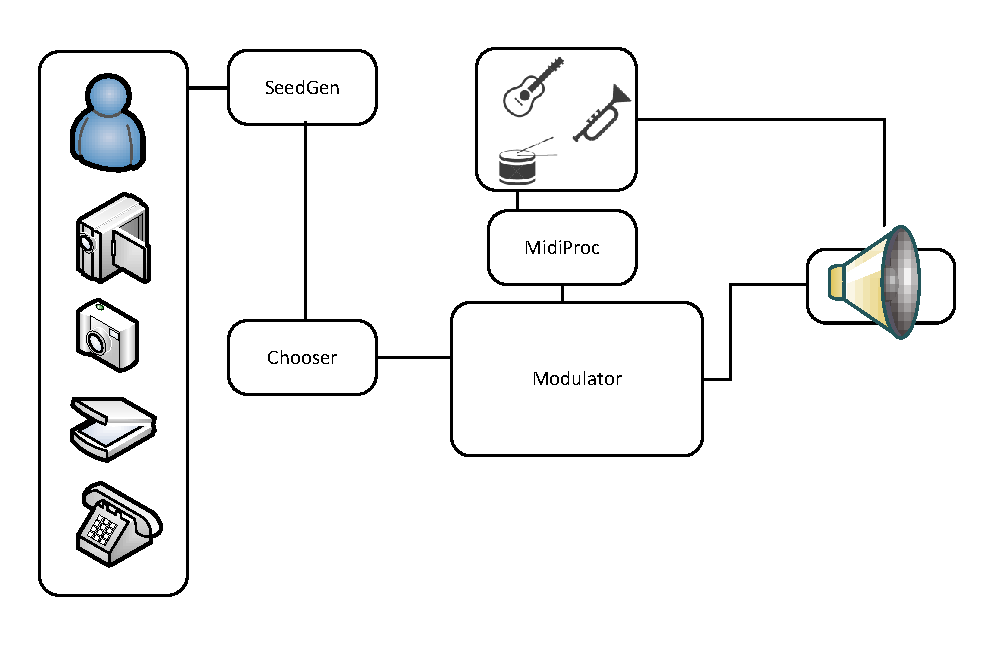
\includegraphics[width=0.6\textwidth]{concept.pdf}
       \label{fig:hans}
\end{figure}


\end{frame}

\section{First Session}
\subsection{Recording Environment}
\begin{frame}
\frametitle{First Session}
\framesubtitle{Recording Environment}

\begin{columns}
    \begin{column}{0.48\textwidth}
        \begin{itemize}
        \item do-it-yourself approach
        \begin{itemize}
        \item in a flat with headphones and mixer
        \item self-build musical instruments        
        \end{itemize}
        \item chaotic set-up
        \item guest participants
        \end{itemize}      
    \end{column}
    \begin{column}{0.48\textwidth}
       \begin{figure}[h!]
       \centering
       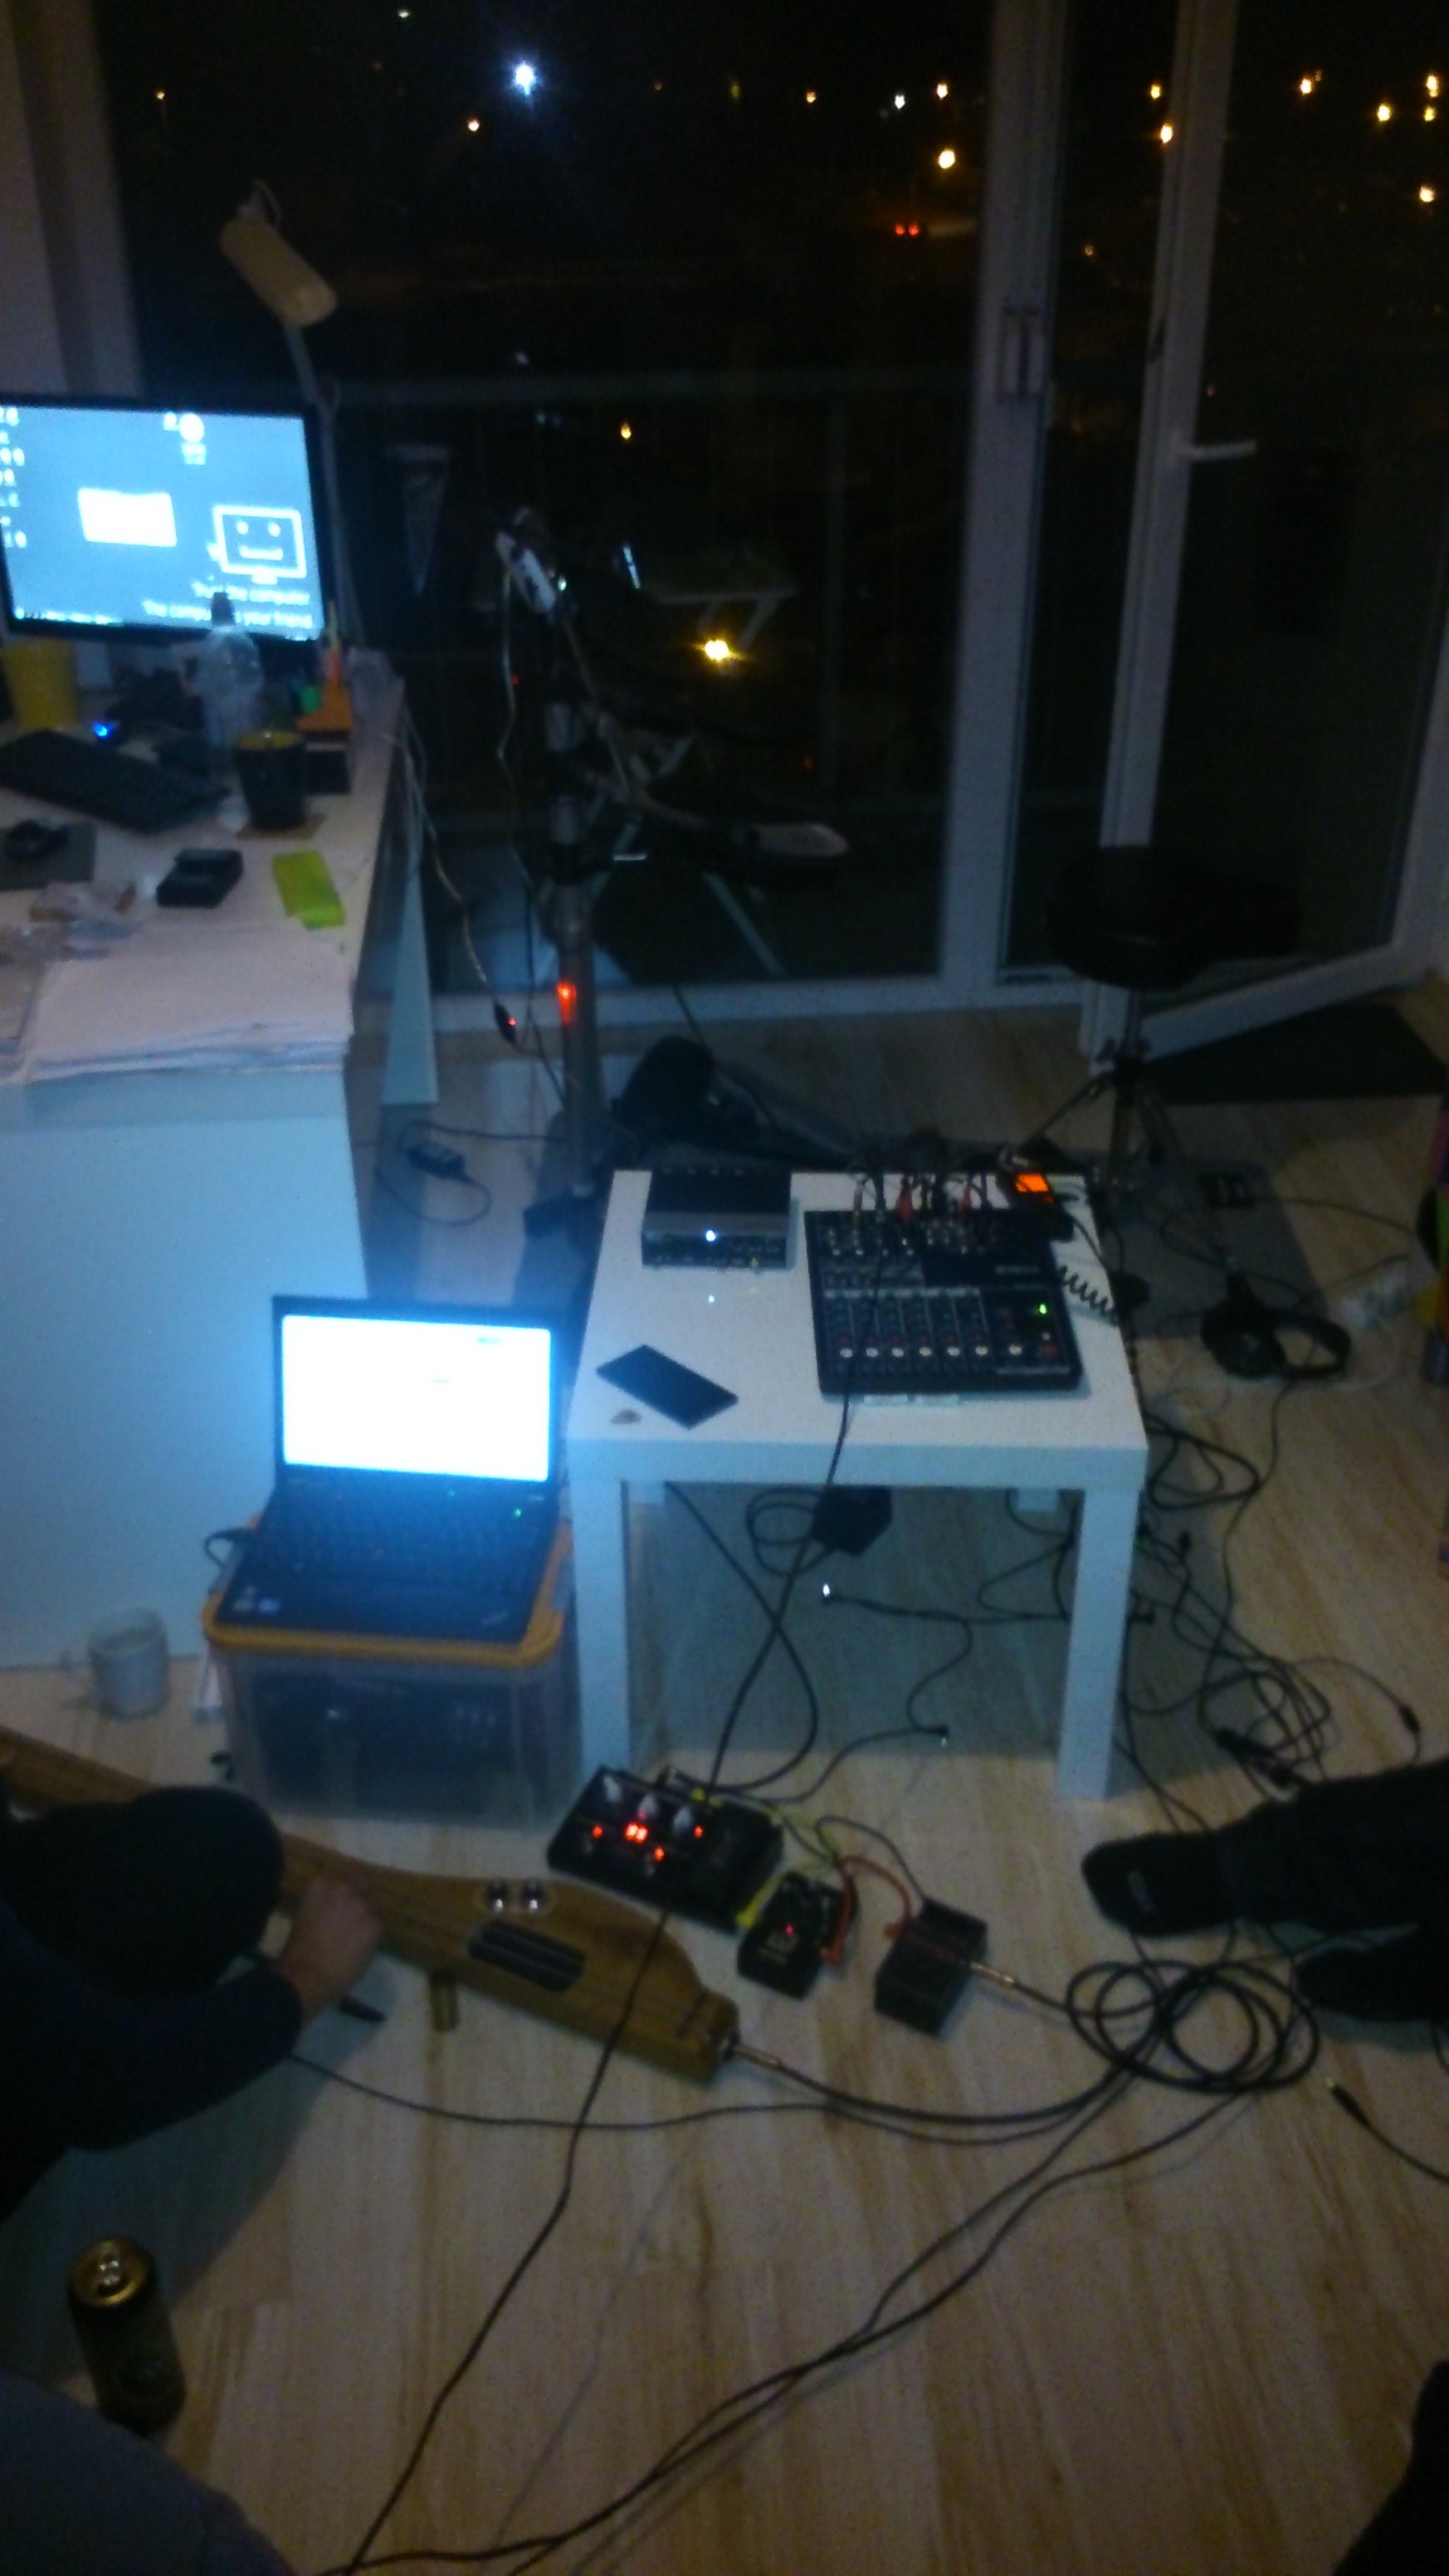
\includegraphics[width=0.75\textwidth]{DSC_0402.jpg}
       \label{fig:rec_env}
       \end{figure}
    \end{column}
\end{columns}

\end{frame}

\subsection{Demo}
\begin{frame}
\frametitle{First Session}
\framesubtitle{Demo}

\begin{itemize}
\item we recorded the whole session (three and a half hour long)
\item we chose a 15 minutes continuous excerpt as a demonstration of HANS
\item we uploaded to public sound-sharing site, Soundcloud
\begin{itemize}
\item independent distribution
\item \url{https://soundcloud.com/leait/hans-0000001}
\end{itemize}
\end{itemize}

\end{frame}

\section{The Cover Art}
\begin{frame}
\frametitle{The Cover Art}

\begin{columns}
    \begin{column}{0.48\textwidth}
        \begin{itemize}
        \item chaotic colorization in association with punk culture
        \item computer aided image manipulation
        \item computer science associations
        \begin{itemize}
        \item fractals
        \item neon colors
        \item computer screens
        \item inverse binary composition
        \end{itemize}
       	\end{itemize}
    \end{column}
    \begin{column}{0.48\textwidth}
        \begin{figure}[h!]
        \centering
        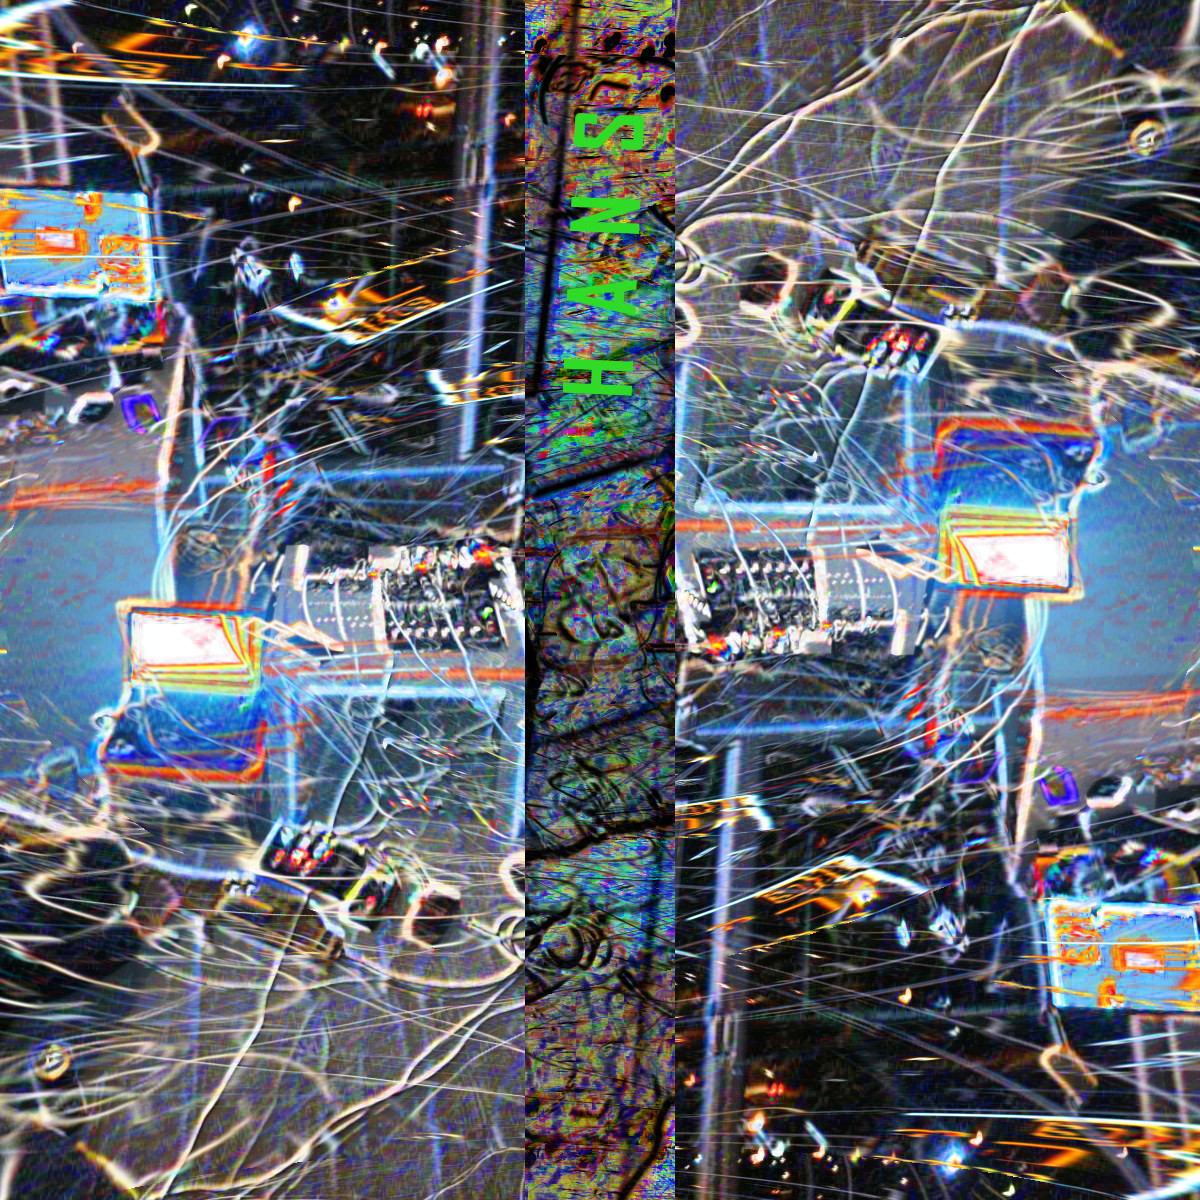
\includegraphics[width=0.9\textwidth]{hans_neon_1x2.jpg}
        \label{fig:cover_art}
        \end{figure}
    \end{column}
\end{columns}

\end{frame}

\section{Feedback}
\begin{frame}
\frametitle{Feedback}

\begin{itemize}
\item ``The music of HANS is \textbf{awesome} to get home after heavy drinking.''
\item ``I \textbf{can not process} the experience.''
\item ``I listened to it fully only once. \textbf{Not any more}.''
\end{itemize}
\end{frame}

\section{Summary}
\subsection{Conclusion \& Future Work}
\begin{frame}
\frametitle{Summary}
\framesubtitle{Conclusion \& Future Work}

\begin{itemize}
\item Conclusion
\begin{itemize}
\item We created an audible piece of conceptual art
\item Output: recording, cover art \& software
\end{itemize}
\item Future Work
\begin{itemize}
\item improving HANS
\item rehearsals
\item performances
\item involve other \textit{performers}
\end{itemize}
\end{itemize}

\vfill
\begin{center}
\LARGE \textbf{Thank you for your attention!}
\end{center}

\end{frame}

\end{document}